% ============================================================
%  TERM PROJECT – PROPOSAL (template)
%  Databases · THGA Bochum
%
%  How to use:
%    1. Copy this folder into your own repository.
%    2. Replace every  <<< ... >>>  placeholder with your content.
%    3. Build with  `make`  (see the Makefile / README).
%    4. Send the resulting PDF to the lecturer and wait for approval.
% ============================================================
\documentclass[11pt,a4paper]{article}

\usepackage{thga-db}
\usepackage{caption}   % enables \captionof inside minipages

% ----- Fill in your metadata -------------------------------
\renewcommand{\thgaKurs}{Databases}
\renewcommand{\thgaDatum}{Summer Term 2026}
\newcommand{\authorName}{Ahmad Hoteit}
\newcommand{\projectTitle}{Fit Tracker}

\begin{document}
\thispagestyle{empty}
\thgaTitel{Term Project – Proposal}{\projectTitle}

\begin{infobox}
\textbf{Author:} \authorName \\
\textbf{Module:} Introduction to Database Management Systems · THGA Bochum \\
\textbf{Submitted to:} Stephan Bökelmann · \href{mailto:sboekelmann@ep1.rub.de}{sboekelmann@ep1.rub.de} \\
\textbf{Target size:} about 6 pages
\end{infobox}

\begin{infobox}
\textbf{Every figure must be explained in the running text.} A figure never
stands on its own: refer to it by number and say what it shows -- e.g.
``Figure~\ref{fig:er} shows the ER model of \dots''.

Every figure below is \texttt{example-figure.jpg}, a dummy image shipped with
this template. Photograph or scan your own sketch, drop the file next to
\texttt{proposal.tex}, and point \texttt{\textbackslash includegraphics} at it:
\begin{quote}
\texttt{\textbackslash includegraphics[width=0.85\textbackslash linewidth]\{er-sketch.jpg\}}
\end{quote}
The \texttt{width} option scales the image to a fraction of the text width; the
file extension may be omitted. Keep the \texttt{\textbackslash caption} and the
\texttt{\textbackslash label} as they are.
\end{infobox}

% ============================================================
\section{Application domain and motivation}
% ============================================================
Fit Tracker is a self-hosted database application designed to record and manage strength training sessions. It solves the problem of tracking gym progress by replacing disorganized pen-and-paper logs and bloated, expensive commercial fitness apps. The primary users are gym-goers and strength training enthusiasts who want a fast, lightweight, and private way to log their workouts.

Usage Scenarios:

a- Logging a Session: A user finishes a set of bench presses at the gym. They open the Fit 
Tracker desktop client, create a new workout entry for the day, select "Bench Press" from the exercise dictionary, and log the exact weight, sets, and repetitions performed to ensure they are hitting their progressive overload targets.

b- Reviewing History: Before starting a workout, a user queries their past sessions to check what weight they lifted for squats the previous week, allowing them to know exactly how much weight to load on the bar for their current session.

% ============================================================
\section{Data model -- ER sketch}
% ============================================================

\begin{figure}[ht]
  \centering
  % Swap example-figure.jpg for your own file, e.g. er-sketch.jpg
  % (a photographed hand drawing is fine).
  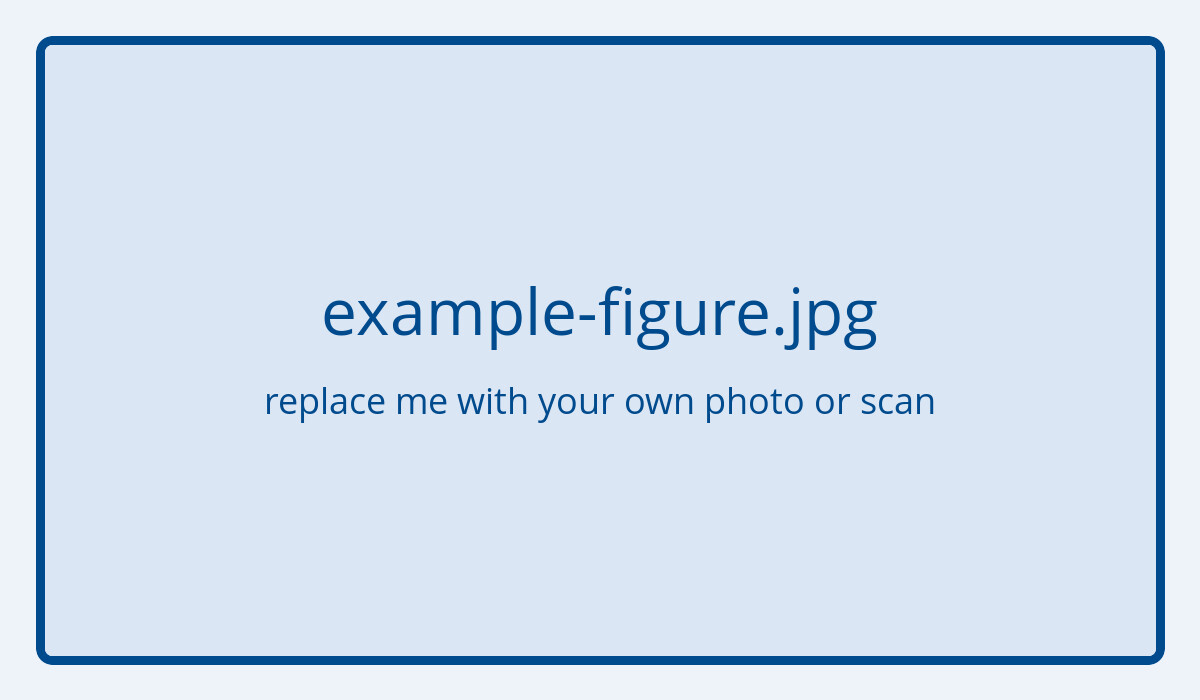
\includegraphics[width=0.85\linewidth]{example-figure.jpg}
  \caption{ER sketch of the Fit Tracker data model: entity types, key
  attributes, relationships and cardinalities (at least one N:M).}
  \label{fig:er}
\end{figure}

Figure~\ref{fig:er} shows the ER model for the Fit Tracker system. The central
entity types are User, Workout, and Exercise. Their primary key attributes are
user\_id, workout\_id, and exercise\_id, respectively. A User can have multiple
Workouts (a 1:N relationship). The core of the system is the N:M relationship
between Workout and Exercise: a single workout session includes multiple exercises,
and a specific exercise is performed across many workouts. This N:M relationship is
resolved via the WorkoutExercise entity, which captures the specific details of
each performance (sets, reps, and weight).

% ============================================================
\section{From model to schema}
% ============================================================

The relational schema for the Fit Tracker system is derived as follows:

\begin{itemize}
  \item \texttt{User}(\underline{user\_id}, username, email, created\_at)
  \item \texttt{Exercise}(\underline{exercise\_id}, name, target\_muscle, description)
  \item \texttt{Workout}(\underline{workout\_id}, \emph{user\_id}, workout\_date, notes)
  \item \texttt{WorkoutExercise}(\underline{workout\_exercise\_id}, \emph{workout\_id}, \emph{exercise\_id}, sets, reps, weight\_kg)
\end{itemize}

\textbf{Normalisation.} The schema is in the Third Normal Form (3NF) because all non-key attributes depend entirely on the primary key of their respective tables. Furthermore, there are no transitive dependencies between non-key attributes, and the N:M relationship is fully resolved via the junction table to prevent redundant data.

% ============================================================
\section{API design}
% ============================================================

The planned FastAPI endpoints for the Fit Tracker system are listed below. The read operations include necessary aggregations, while all write operations are secured to prevent unauthorized modifications.

\renewcommand{\arraystretch}{1.5}
\begin{tabularx}{\linewidth}{@{}p{2cm}p{6cm}X@{}}
\toprule
\textbf{Method} & \textbf{Path} & \textbf{Purpose} \\
\midrule
\texttt{GET}  & \texttt{/users/\{user\_id\}/workouts} & Reads workout history (JOINs Workout, WorkoutExercise, and Exercise to aggregate full session details). \\
\texttt{GET}  & \texttt{/exercises} & Reads the static dictionary of available exercises. \\
\texttt{POST} & \texttt{/workouts} & Creates a new workout session (requires X-API-Key). \\
\texttt{POST} & \texttt{/workouts/\{workout\_id\}/exercises} & Logs specific sets, reps, and weights to an existing workout (requires X-API-Key). \\
\bottomrule
\end{tabularx}


% ============================================================
\section{Frontend prototype (hand sketches)}
% ============================================================

The frontend is a lightweight desktop application built using Python and Tkinter. This framework is recommended for its straightforward native GUI components and ability to be easily packaged into a \texttt{.deb} installer. The frontend is delivered as a \texttt{.deb} installer and asks for the API URL (including the specific port assigned on the lecture server) and the X-API-Key in a connection dialog at startup.

% Each \includegraphics below still points at the dummy example-figure.jpg.
% Swap in your own file per screen, e.g. {fe-connect.jpg}, and keep the \captionof.
\begin{figure}[ht]
\centering
\begin{minipage}[t]{0.47\linewidth}\centering
  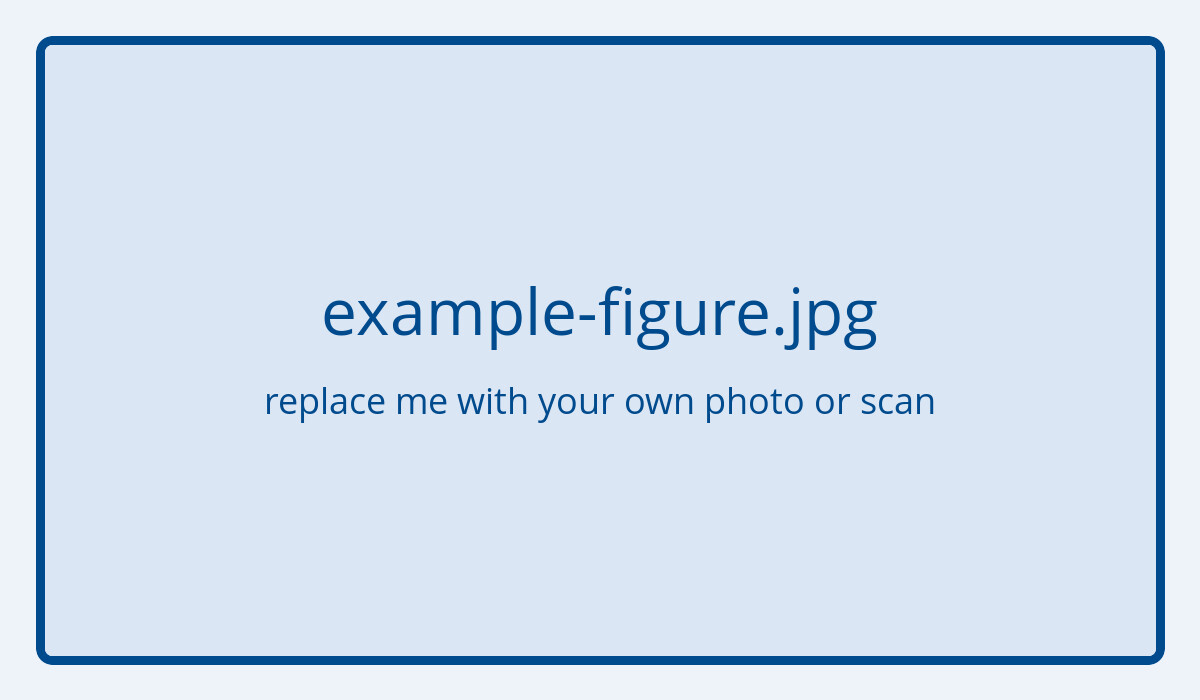
\includegraphics[width=\linewidth]{example-figure.jpg}
  \captionof{figure}{Startup connection dialog: API URL + X-API-Key.}
  \label{fig:fe-connect}
\end{minipage}\hfill
\begin{minipage}[t]{0.47\linewidth}\centering
  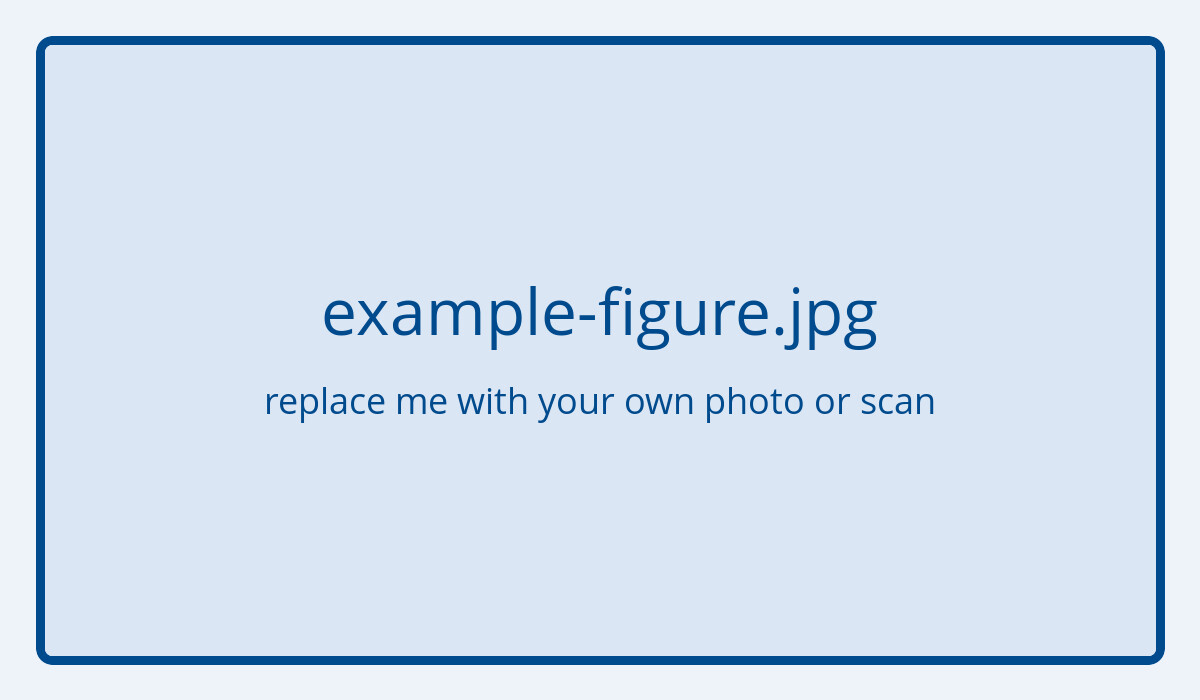
\includegraphics[width=\linewidth]{example-figure.jpg}
  \captionof{figure}{Main screen: Workout history list, calls \texttt{GET /users/\{user\_id\}/workouts}.}
  \label{fig:fe-main}
\end{minipage}

\vspace{1em}

\begin{minipage}[t]{0.47\linewidth}\centering
  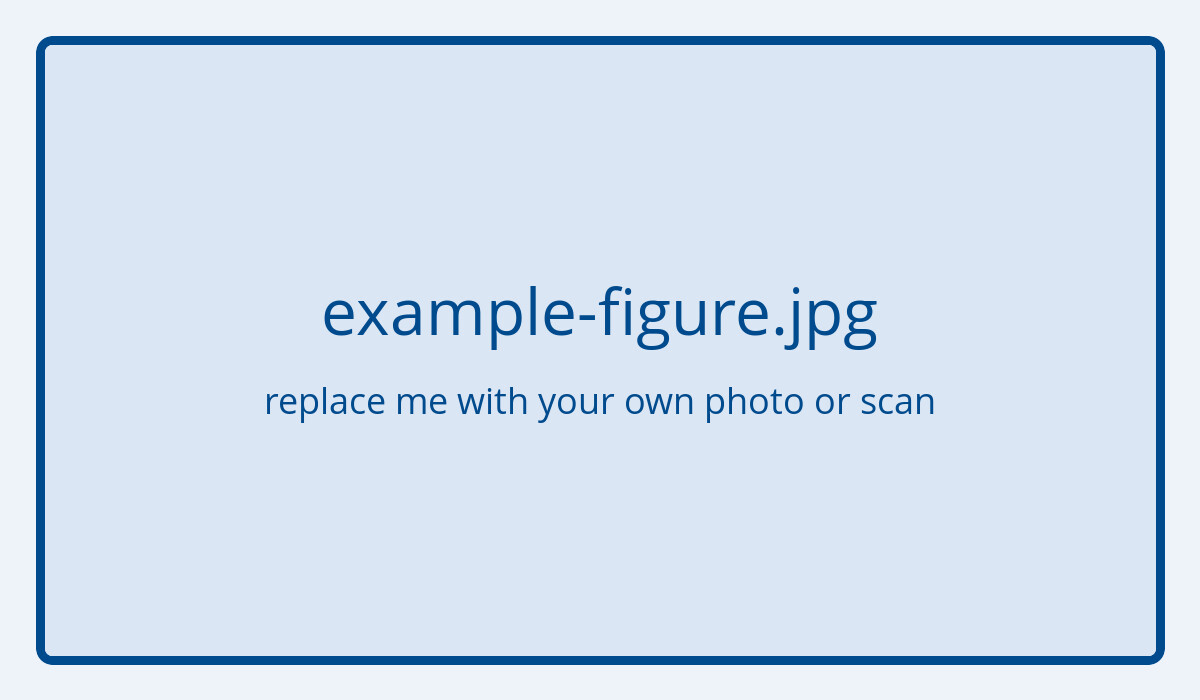
\includegraphics[width=\linewidth]{example-figure.jpg}
  \captionof{figure}{Detail form: Log new session and sets, calls \texttt{POST /workouts} and \texttt{POST /workouts/\{workout\_id\}/exercises}.}
  \label{fig:fe-detail}
\end{minipage}\hfill
\begin{minipage}[t]{0.47\linewidth}\centering
  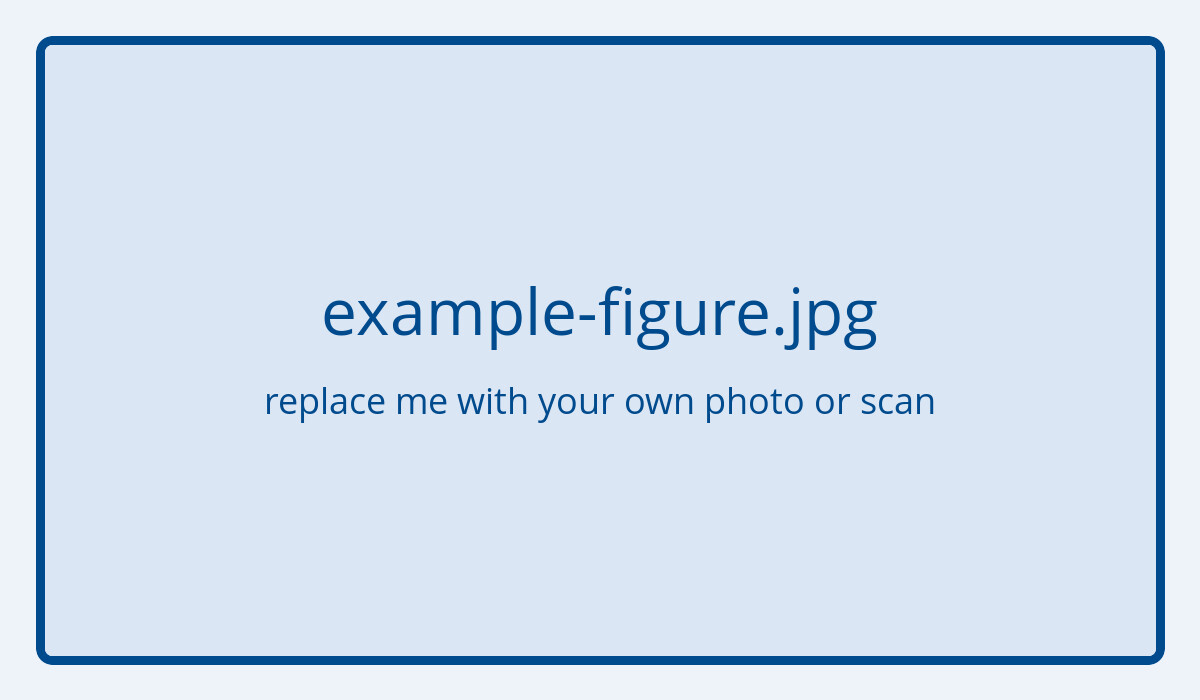
\includegraphics[width=\linewidth]{example-figure.jpg}
  \captionof{figure}{Exercise Dictionary: Lists available movements, calls \texttt{GET /exercises}.}
  \label{fig:fe-second}
\end{minipage}
\end{figure}

Figures~\ref{fig:fe-connect}--\ref{fig:fe-second} show the four screens of the prototype. Figure~\ref{fig:fe-connect} shows the connection dialog that collects the API URL and X-API-Key at startup; Figure~\ref{fig:fe-main} shows the main screen displaying the user's workout history and the read endpoint it calls; Figure~\ref{fig:fe-detail} shows the form used to log a new workout along with its specific sets and the write endpoints it calls; and Figure~\ref{fig:fe-second} shows the exercise dictionary screen displaying target muscles.

% ============================================================
\section{Operation with Docker Compose}
% ============================================================

The system is containerized using Docker to ensure a consistent deployment environment. The \texttt{docker-compose.yml} file orchestrates two primary services:
\begin{itemize}
  \item \textbf{postgres}: The database service running the PostgreSQL image, which persists data via Docker volumes to ensure no workout records are lost.
  \item \textbf{api}: The backend service running the FastAPI application, which connects internally to the \texttt{postgres} container.
\end{itemize}

All sensitive configuration details, including the database credentials and the \texttt{X-API-Key}, are stored securely in a \texttt{.env} file. This file is explicitly excluded from version control to maintain security.

For deployment on the lecture server, the repository is cloned and the \texttt{.env} file is populated with the production credentials. The containers are then built and started in detached mode using Docker Compose. To make the backend accessible without conflicts, the internal port of the \texttt{api} container is mapped directly to the specific port assigned to this project on the lecture server.


% ============================================================
\section{Scope, milestones and risks}
% ============================================================

\textbf{Scope.} The Fit Tracker system is scoped to exactly 4 relational tables (User, Exercise, Workout, WorkoutExercise) and 4 FastAPI endpoints (two GET reads and two POST writes).

\textbf{Milestones and schedule.} The project will be executed in a single intensive development sprint following the conclusion of examinations, totaling roughly 40 hours of work.

\renewcommand{\arraystretch}{1.2}
\begin{tabularx}{\linewidth}{@{}p{2.5cm}Xp{1.8cm}@{}}
\toprule
\textbf{Sprint Date} & \textbf{Milestone} & \textbf{Est. hours} \\
\midrule
29.07.2026 & Schema setup, Docker configuration, and seed data ready & 8 \\
30.07.--31.07. & API read/write implementation, protected by X-API-Key & 12 \\
01.08.--02.08. & Frontend operates core endpoints, \texttt{.deb} packaging & 10 \\
03.08.--04.08. & Acceptance testing, final documentation, and demo video & 10 \\
\bottomrule
\end{tabularx}

\textbf{Risks.} 
There are two main risks that could impact the project:
\begin{itemize}
  \item \textbf{Deployment constraints:} Port conflicts or network permission issues could arise when deploying the backend containers to the shared lecture server.
  \item \textbf{Packaging complexities:} Unexpected system dependencies or missing libraries might cause failures when packaging the Python/Tkinter frontend into a standalone \texttt{.deb} installer.
\end{itemize}



% ============================================================
\section{Acceptance criteria and testing}
% ============================================================

The system is considered ``done and correct'' when all constraints are enforced at the database level, the API accurately handles all defined requests securely, and the frontend successfully installs and connects to the backend in a production-like environment.

\textbf{Acceptance criteria.} 
\begin{itemize}[topsep=2pt]
  \item A workout or exercise record that violates a database constraint (e.g., negative weight) is rejected (API returns 422/400).
  \item \texttt{GET /users/\{user\_id\}/workouts} returns the correct aggregated session details (verifying the JOIN between Workout, WorkoutExercise, and Exercise).
  \item Write endpoints (\texttt{POST /workouts} and \texttt{POST /workouts/\{workout\_id\}/exercises}) without a valid X-API-Key are refused (API returns 401/403).
  \item The Python/Tkinter frontend installs cleanly via the \texttt{.deb} package and successfully connects to the lecture server port.
\end{itemize}

\textbf{Test plan.} 
\begin{itemize}[topsep=2pt]
  \item \textbf{Database:} Verify that PK/FK constraints (ensuring orphan workout exercises cannot exist) and NOT NULL constraints (e.g., workout\_date, target\_muscle) are strictly enforced.
  \item \textbf{API:} Automated endpoint tests covering both the happy path and error cases, executed with \texttt{pytest} and FastAPI's \texttt{TestClient} against a clean test database.
  \item \textbf{Business rule:} To address the primary risks, a clean-room installation test will verify the \texttt{.deb} package dependencies, and a deployment test will confirm the API binds successfully to the assigned lecture server port without configuration conflicts.
\end{itemize}

\vspace{1em}
\begin{infobox}
\textbf{Effort budget:} the whole term project (system, documentation and video)
should fit into roughly \textbf{40\,h of work} over at most \textbf{2 months}.
Keep your scope within that budget.
\end{infobox}

\end{document}
